\chapter{Experiment Result}
\label{chap:ExperimentResult}

\section{Comparison of Computational Efficiency and Resource Usage}
\label{sec:ComparisonofComputationalEfficiencyandResourceUsage}
\begin{table*}[htbp]
    \caption{Comparison of Computational Efficiency and Resource Usage}
    \centering
    \begin{tabularx}{\textwidth}{|X|X|X|X|}
        \hline
        Method & Means of Photography & Environment Creation Time (from images) & Need for specialized expertise \\
        \hline
        NeRF2Real [5] & Smartphone camera & 2-3 hours & Yes \\
        \hline
        Matterport3D [6] & Camera rig & Several days & Yes \\
        \hline
        Our method & Smartphone camera & 1-2 hours & No \\
        \hline
    \end{tabularx}
    \label{tab:ComparisonofComputationalEfficiencyandResourceUsage}
\end{table*}

\singlespacing
The Table.\ref{tab:ComparisonofComputationalEfficiencyandResourceUsage} elucidated in the table underscores pronounced disparities in computational efficiency and resource utilization across three paradigms for virtual environment creation: NeRF2Real, Matterport3D, and Our Method. Each paradigm employs distinct photographic techniques and varies in temporal commitments for environment genesis, alongside requisites for specialized acumen. 
\singlespacing
NeRF2Real, deploying a smartphone camera, strikes a nuanced equilibrium between alacrity and technical intricacy. It necessitates roughly 2-3 hours for creating an environment, apt for compact spaces. Nonetheless, the prerequisite of eight NVIDIA V100 GPUs and specialized knowledge renders it less attainable for the layperson. This method is propitious for scenarios seeking a harmonious blend of efficacy and professional caliber, yet its dependence on advanced GPUs and technical prowess curtails its widespread applicability.
\singlespacing
Conversely, Matterport3D markedly prolongs the environmental creation process, spanning several days. Predicated on a camera rig, it demands not only specialized apparatus but also expert intervention. Its protracted creation interval and need for specialized rigging augment the precision and intricacy of the resultant environments, rendering it exemplary for professional-grade simulations. However, its complexity and resource exigencies render it impracticable for casual or resource-constrained entities.
\singlespacing
Our method distinguishes itself as the most user-centric and accessible alternative. Leveraging a smartphone camera, it requires a mere 1-2 hours for environment creation, eschewing the need for specialized expertise. This method democratizes virtual environment creation, rendering it attainable for individuals devoid of technical backgrounds or significant resources. Its simplicity and cost-efficiency designate it as the quintessential choice for casual users or those desiring a straightforward pathway to environment simulation.
\singlespacing
In summation, juxtaposing these tripartite methodologies unveils a spectrum of options for virtual environment creation, each catering to divergent requisites and resource availabilities. NeRF2Real presents a median path with moderate efficiency and complexity; Matterport3D offers high-fidelity environments at the expense of substantial resources; and Our method emerges as the most accessible and user-friendly, accommodating an expansive array of users.



\section{Yolo Result}
\label{sec:YoloResult}

\begin{table*}[htbp]
    \caption{Comparison of Object Recognition Performance in Real and Virtual Environments}
    \centering
    \begin{tabularx}{\textwidth}{|X|X|X|X|X|}
        \hline
        Environment & TP & FP & FP & F1-score \\
        \hline
        Kiosk & 2 & 1 & 0 & 80\% \\
        \hline
        Research Building & 5 & 0 & 0 & 100\% \\
        \hline
    \end{tabularx}
    \label{tab:ComparisonofObjectRecognitionPerformanceinRealandVirtualEnvironments}
\end{table*}
\begin{figure}[htbp]
  \centering
  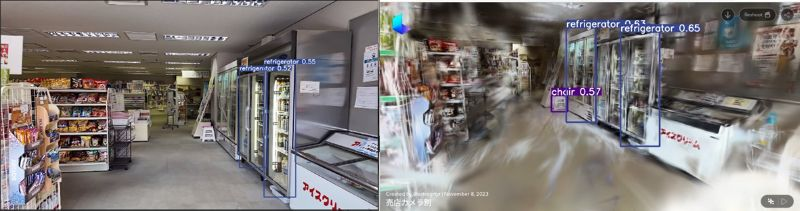
\includegraphics[scale=0.5]{./Figure/Object Recognition at the University of Aizu Kios}
  \caption{Object Recognition at the University of Aizu Kios}
  \label{fig: Object Recognition at the University of Aizu Kios}
\end{figure}
This study compared the performance of object recognition models in real-world and virtual environments and evaluated the agreement rate between these settings. This analysis shows that the match rate is over 80\%, indicating that the virtual environment effectively reflects the real-world scenario. Specifically, the object recognition models showed different performance in different environments. In the kiosk environment, the model had two true positives (TP), one false positive (FP), no false negatives (FN), and an F1 score of 80\%. In contrast, in a lab environment, the model achieved a perfect F1 score of 100\% with 5 true positives and no false positives or negatives. These results suggest that the performance of object detection models varies greatly depending on the environment, and is particularly influenced by the complexity of the setting and the diversity of objects present. This paragraph compares the performance of object recognition models in real-world and virtual environments and highlights the variation in performance in different environments(see Fig.\ref{fig: Object Recognition at the University of Aizu Kios}).
\singlespacing
In addition, we have included the results of YOLO (You Only Look Once) object detection in \ref{tab:ComparisonofObjectRecognitionPerformanceinRealandVirtualEnvironments}. This inclusion provides a comprehensive view of the effectiveness of different models in object detection tasks within these environments. The YOLO model's results further validate our findings and offer an in-depth perspective on the capabilities and limitations of current object detection technologies. This study provides crucial insights supporting the virtual environment's adequacy in accurately replicating the complexities of real-world settings and its validity as a simulation tool in the field of robotics.
\begin{figure}[htbp]
  \centering
  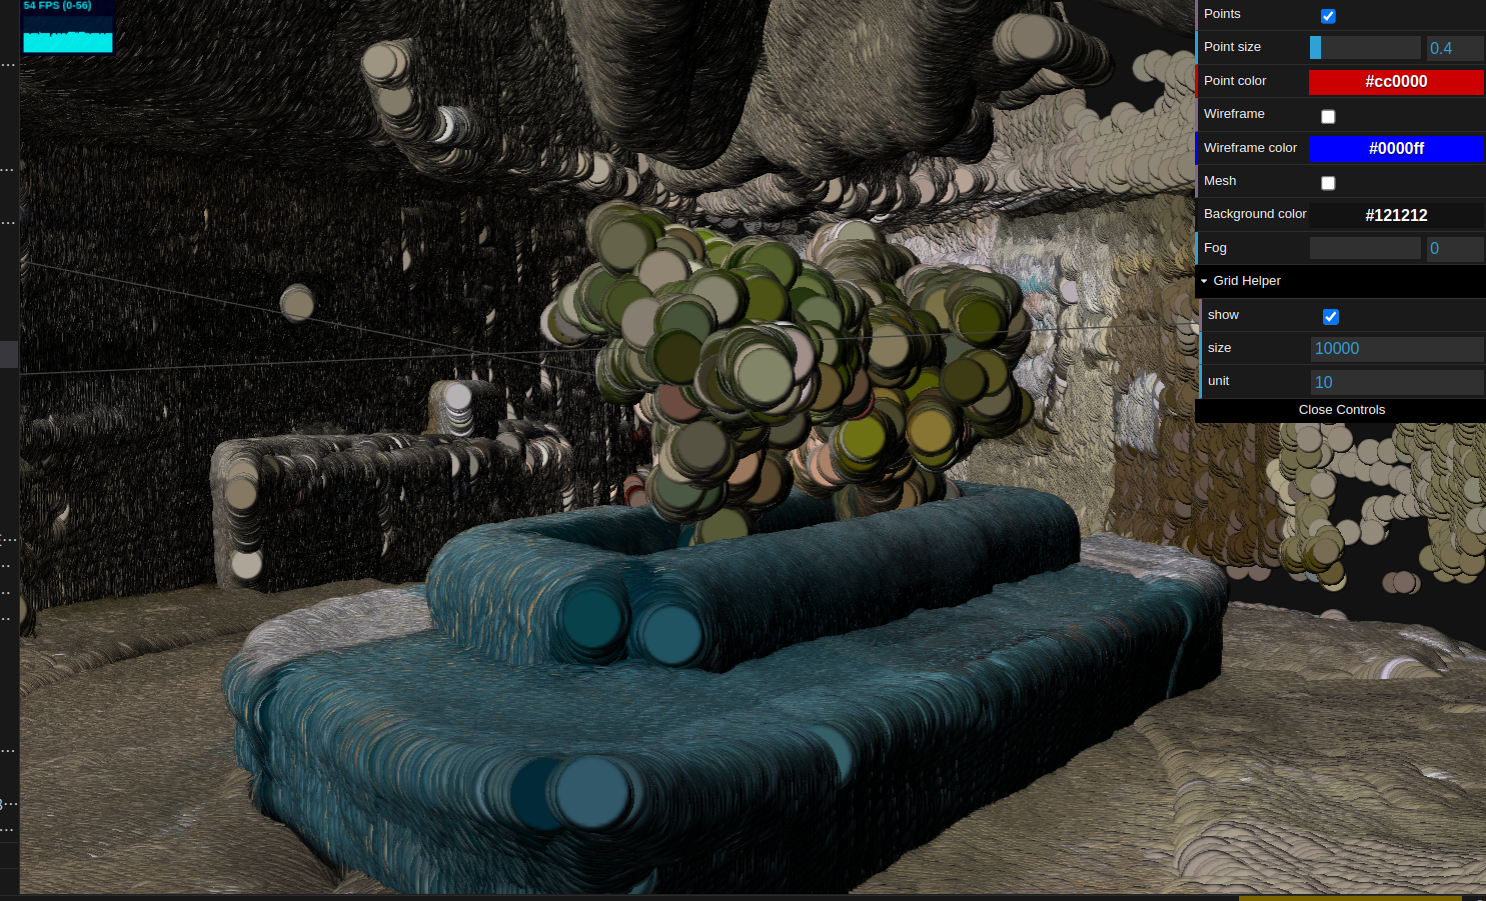
\includegraphics[scale=0.3]{./Figure/研究等の点群.png}
  \caption{Point cloud of the research building generated by Luma AI}
  \label{fig: Point cloud of the research building generated by Luma AI}
\end{figure}
\
\begin{figure}[htbp]
  \centering
  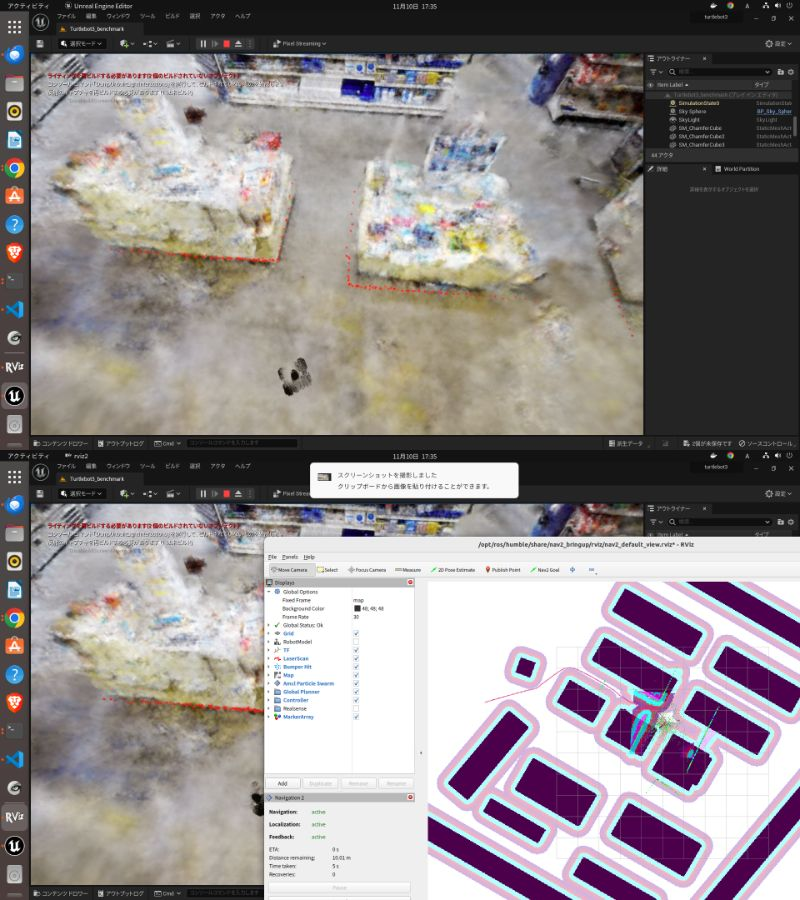
\includegraphics[scale=0.5]{./Figure/n.jpg}
  \caption{Navigation through physical phenomena using point clouds and 3D environments}
  \label{fig:Navigation through physical phenomena using point clouds and 3D environments}
\end{figure}
\section{Navigation2 Result}
\label{sec:Navigation2Result}
This research explores the potential of navigation technology in virtual environments. In particular, focusing on Navigation 2, we combined the point cloud data generated by LumaAI (see. fig\ref{fig: Point cloud of the research building generated by Luma AI}) and Unreal Engine 5's lidar plugin\cite{unrealengine_lidar_plugin} to realize the physical settings of the object. Using this technology, the turtlebot3 waffle model successfully simulated navigation within a virtual environment. This research result represents a major advance in the development of navigation systems in virtual environments.

